% 二体问题综述
% 二体问题|天体运动|质心系|椭圆|轨道

\pentry{中心力场问题\upref{CenFrc}}

由两个质量相近的普通天体组成的系统,称为“二体系统”.

一般情况下,两个天体的体积相比距离可以忽略不计,故可将天体视为质点,研究它们的相对位置的变化关系.

研究两个天体的相对运动,首先需要选取参考点,有两种常用的选择:
\begin{itemize}
\item 以其中一个天体为参考点,研究另一个天体的相对距离和相对速度变化;
\item 以系统质心为参考点,分别研究两个天体相对质心的运动.
\end{itemize}

无外力作用下,系统质心的加速度为零,因此\textbf{由质心为原点建立的参考系是惯性参考系},这也是最常用的参考系.

研究质点系的运动模式的方法,也有两种常用选择:
\begin{itemize}
\item 将每个质点的位置矢量 $\bvec r$ 视为时间 $t$(或其他参数)的未知函数,建立运动微分方程 $\ddot{\bvec r}= \bvec f (t)$,求解该微分方程并代入初值条件,解出运动模式;
\item 将每个质点每个时刻的位置矢量 $\bvec r$ 和动量矢量 $\bvec v$ 视为未知数,由动量定理、角动量定理、能量守恒等建立关于位置矢量和速度矢量的方程组,进而求解.
\end{itemize}
第一种方法最为常见,但是在天体力学和其他力学问题中,很多时候运动微分方程难以求解,因此需综合运用以上两种方法.

\subsection{相似性}
以质心为原点建立坐标系.记天体M的质量为 $m_1$、位置矢量为 $\bvec r_1$,天体N的质量为 $m_2$、位置矢量为$\bvec r_2$.

在此坐标系中,无外力作用下,由\textbf{动量定理}可得
\begin{equation}
\begin{cases}
m_1 \bvec r_1 + m_2 \bvec r_2 = 0\\
m_1 \dot{\bvec r}_1 + m_2 \dot{\bvec r}_2=0
\end{cases}
\end{equation}

可见,两天体的位置矢量和速度矢量分别成固定的比例关系,即两天体相对质心的运动模式是相似的,只需研究其中一个天体,就能得出系统的运动规律.

\subsection{平面性}
 记 $\mu=m_1/m_2$,系统对质心的角动量为
\begin{equation}
\bvec L =\bvec r_1 \times m_1 \dot{\bvec r}_1+ \bvec r_2 \times \dot{\bvec r}_2 = m_1 (1+\mu)\bvec r_1 \times \dot{\bvec r}_1
\end{equation}

\begin{equation}
\dv{\bvec L}{t} = \dot{\bvec r}_1 \times \dot{\bvec r}_1 + \bvec r_1 \times \ddot{\bvec r}_1=\bvec r_1 \times \ddot{\bvec r}_1
\end{equation}

由万有引力定律可得
\begin{equation}\label{ConDB_eq4}
\ddot{\bvec r}_1 = \frac{Gm_2}{|\bvec r_2 - \bvec r_1|^3} \qty(\bvec r_2 - \bvec r_1) = - \frac{Gm_2}{(1+\mu)^2|\bvec r_1|^3}\bvec r_1
\end{equation}
于是
\begin{equation}
\dv{\bvec L}{t} =\bvec r_1 \times \ddot{\bvec r}_1= -\bvec r_1 \times \frac{Gm_2}{(1+\mu)^2|\bvec r_1|^3}\bvec r_1= 0
\end{equation}
即\textbf{角动量守恒}(角动量的方向和模长均守恒).因为角动量垂直于位置矢量和速度矢量所在的平面,故每一时刻位置矢量和速度矢量都在同一平面内,并且加速度矢量也在此平面内.因此,二体系统的运动问题是一个\textbf{平面问题}.

\subsection{轨道方程通解}
记 $k=Gm_1m_2$,则天体M的拉普拉斯-龙格-楞次矢量(L-R-L矢量)可以表示为:
\begin{equation}
\bvec A_1 = m_1\dot{\bvec r}_1 \times \bvec L - \frac{m_1k}{(1+\mu)|\bvec r_1|}\bvec r_1
\end{equation}
二体系统中,L-R-L矢量 $\bvec A_1$ 守恒(此处证明略,可参考词条“拉普拉斯-龙格-楞次矢量\upref{LRLvec}”).

矢量 $\bvec A_1$ 与位置矢量 $r_1$ 作內积,并取坐标形式为极坐标
\begin{equation}\label{ConDB_eq7}
\begin{aligned}
\bvec A_1 \vdot \bvec r_1 &= m_1\dot{\bvec r}_1 \times \bvec L \vdot \bvec r_1 - \frac{m_1k}{(1+\mu)}r_1\\
&= m_1\qty(\bvec r_1 \times \dot{\bvec r}_1)\vdot \bvec L - \frac{m_1k}{(1+\mu)}r_1 \\
&= \frac{L^2-m_1k}{1+\mu}r_1
\end{aligned}
\end{equation}
\begin{figure}[ht]
\centering
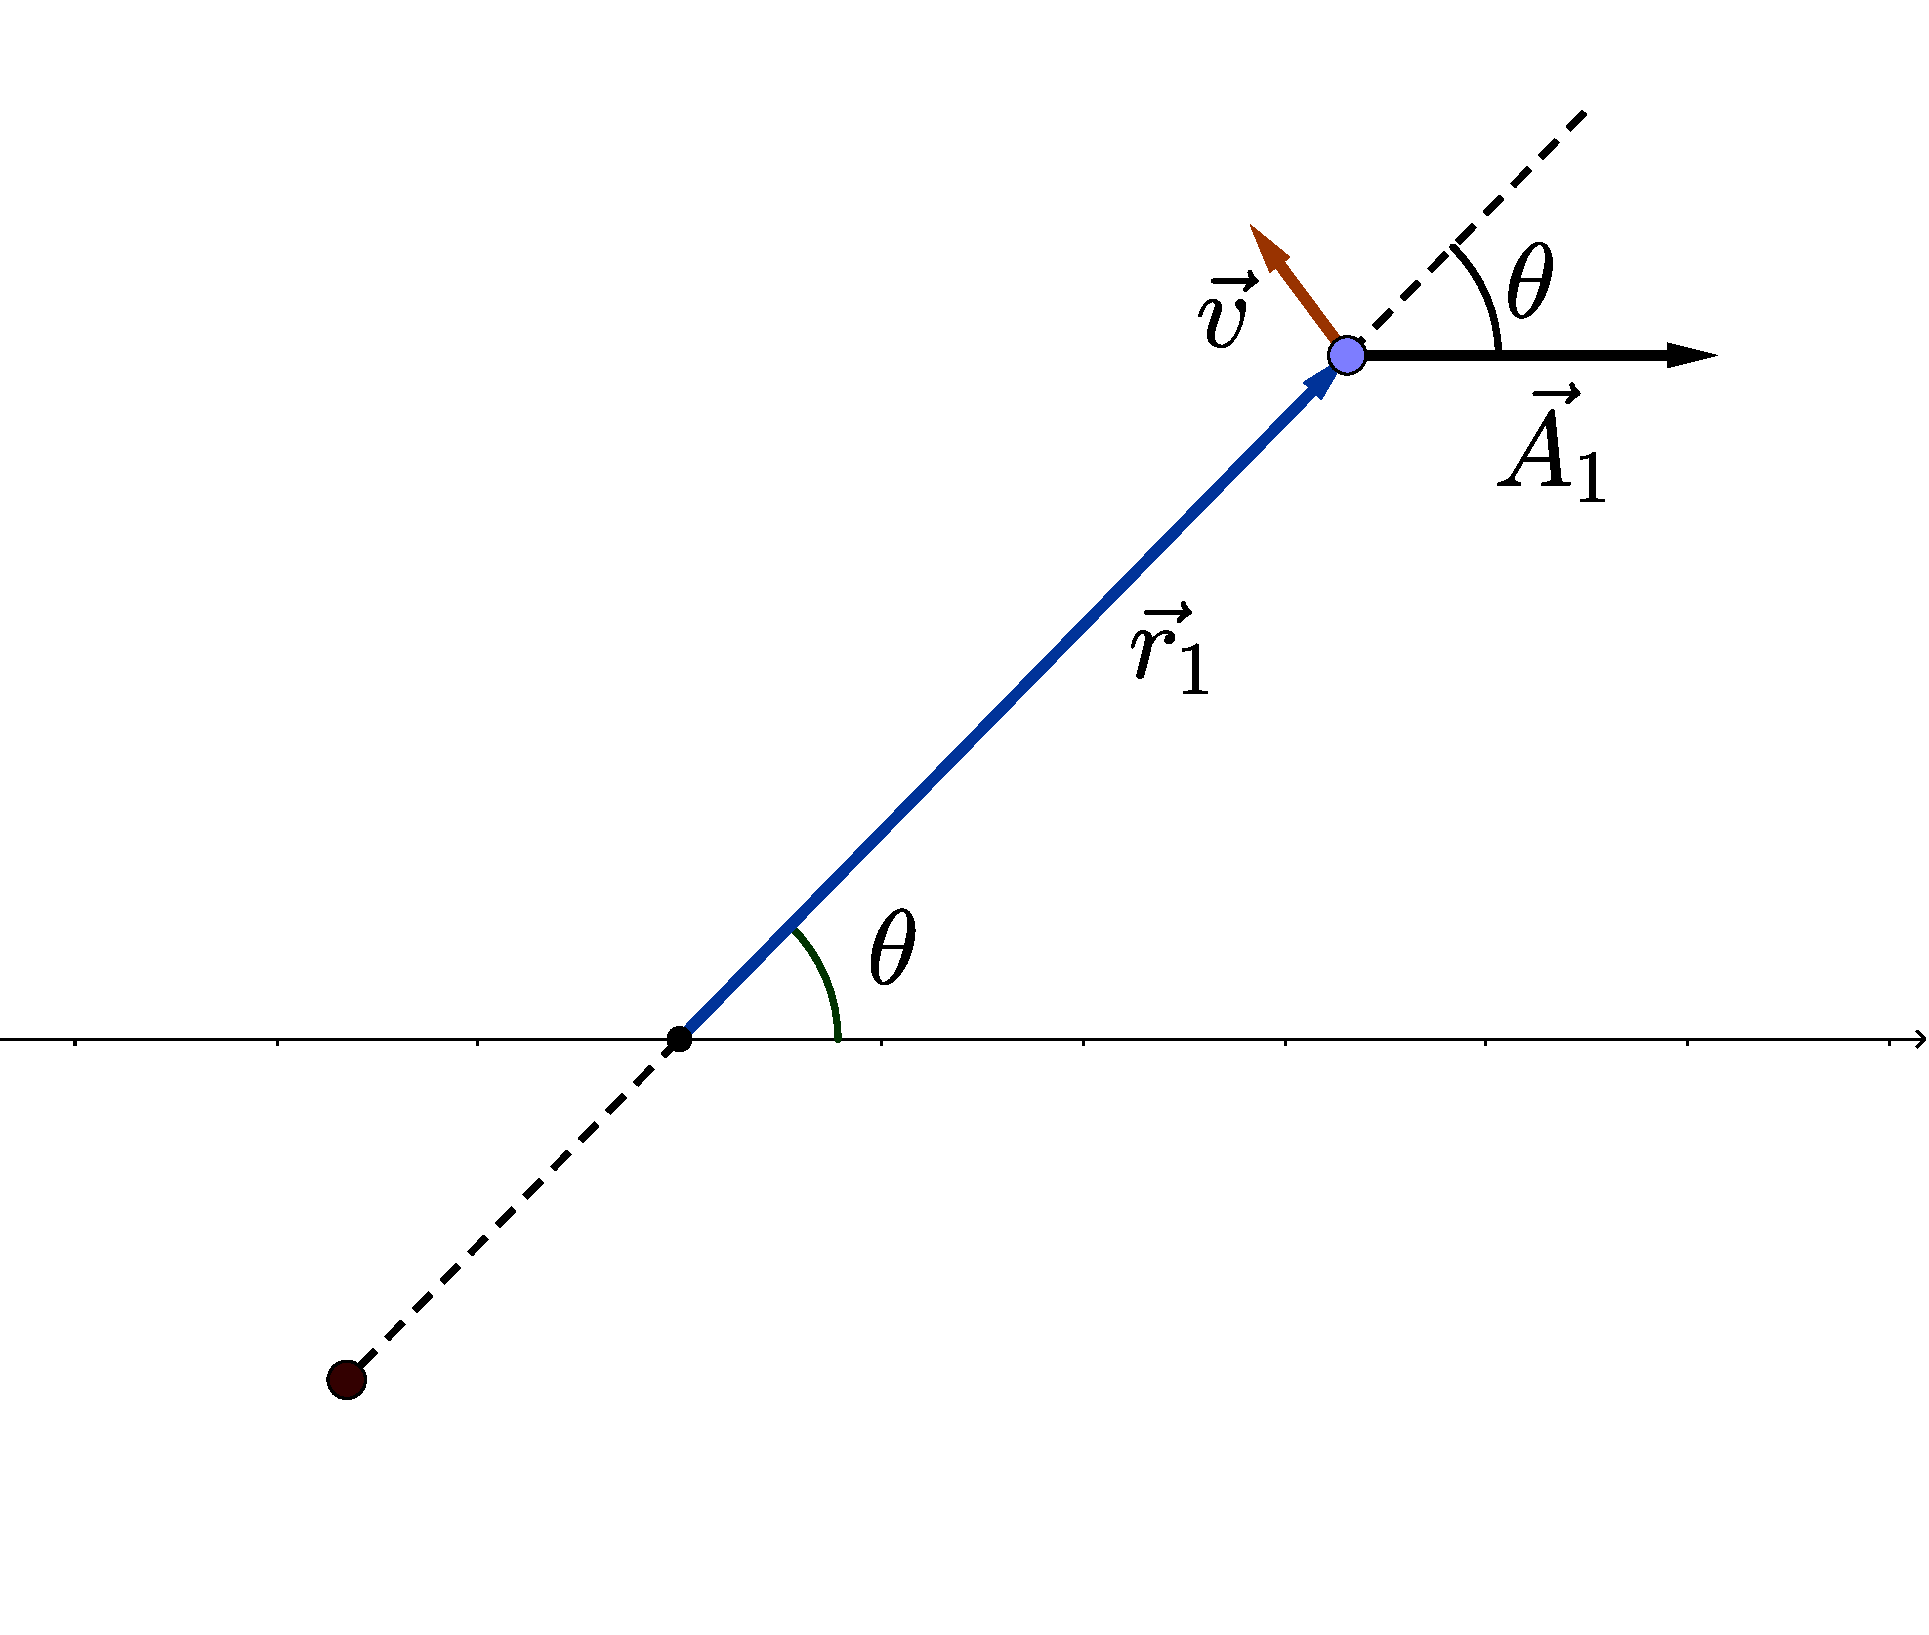
\includegraphics[width=8cm]{./figures/ConDB_1.pdf}
\caption{L-R-L矢量与位置矢量} \label{ConDB_fig1}
\end{figure}

令 $\theta$ 为从矢量 $\bvec A_1$ 转向位置矢量 $\bvec r_1$ 的夹角(极轴与从矢量 $\bvec A_1$ 平行,如\autoref{ConDB_fig1}).则\autoref{ConDB_eq7}可化为
\begin{equation}
A_1r_1\cos\theta = \frac{L^2-m_1k}{1+\mu}r_1
\end{equation}
移项整理可得轨道的极坐标方程
\begin{equation}\label{ConDB_eq9}
r_1=\frac{p}{1+e \cos\theta}
\end{equation}
其中,$p=L^2/(m_1k)$,$e=A_1(1+\mu)/(m_1k)$.

可见天体M的轨迹是圆锥曲线,其偏心率由L-R-L矢量 $\bvec A_1$ 决定.天体N的轨迹与之相似.当两个天体的质量相差悬殊,则大质量的天体运动范围极小,且系统质心非常靠近大质量天体,两天体的相对运动模式则近似为单质点在引力场中的运动(即开普勒问题,恒星—行星运动模式).

通过求解天体M的运动微分方程\autoref{ConDB_eq4} ,也可以得到相同的结果(推导过程参考“开普勒问题\upref{CelBd}”和“轨道方程—比耐公式\upref{Binet}”).

在\autoref{ConDB_fig2} 中展示了二体系统的四种运动轨迹,分别为圆形轨迹、椭圆形轨迹、抛物线形轨迹和双曲线形轨迹.
\begin{figure}[ht]
\centering
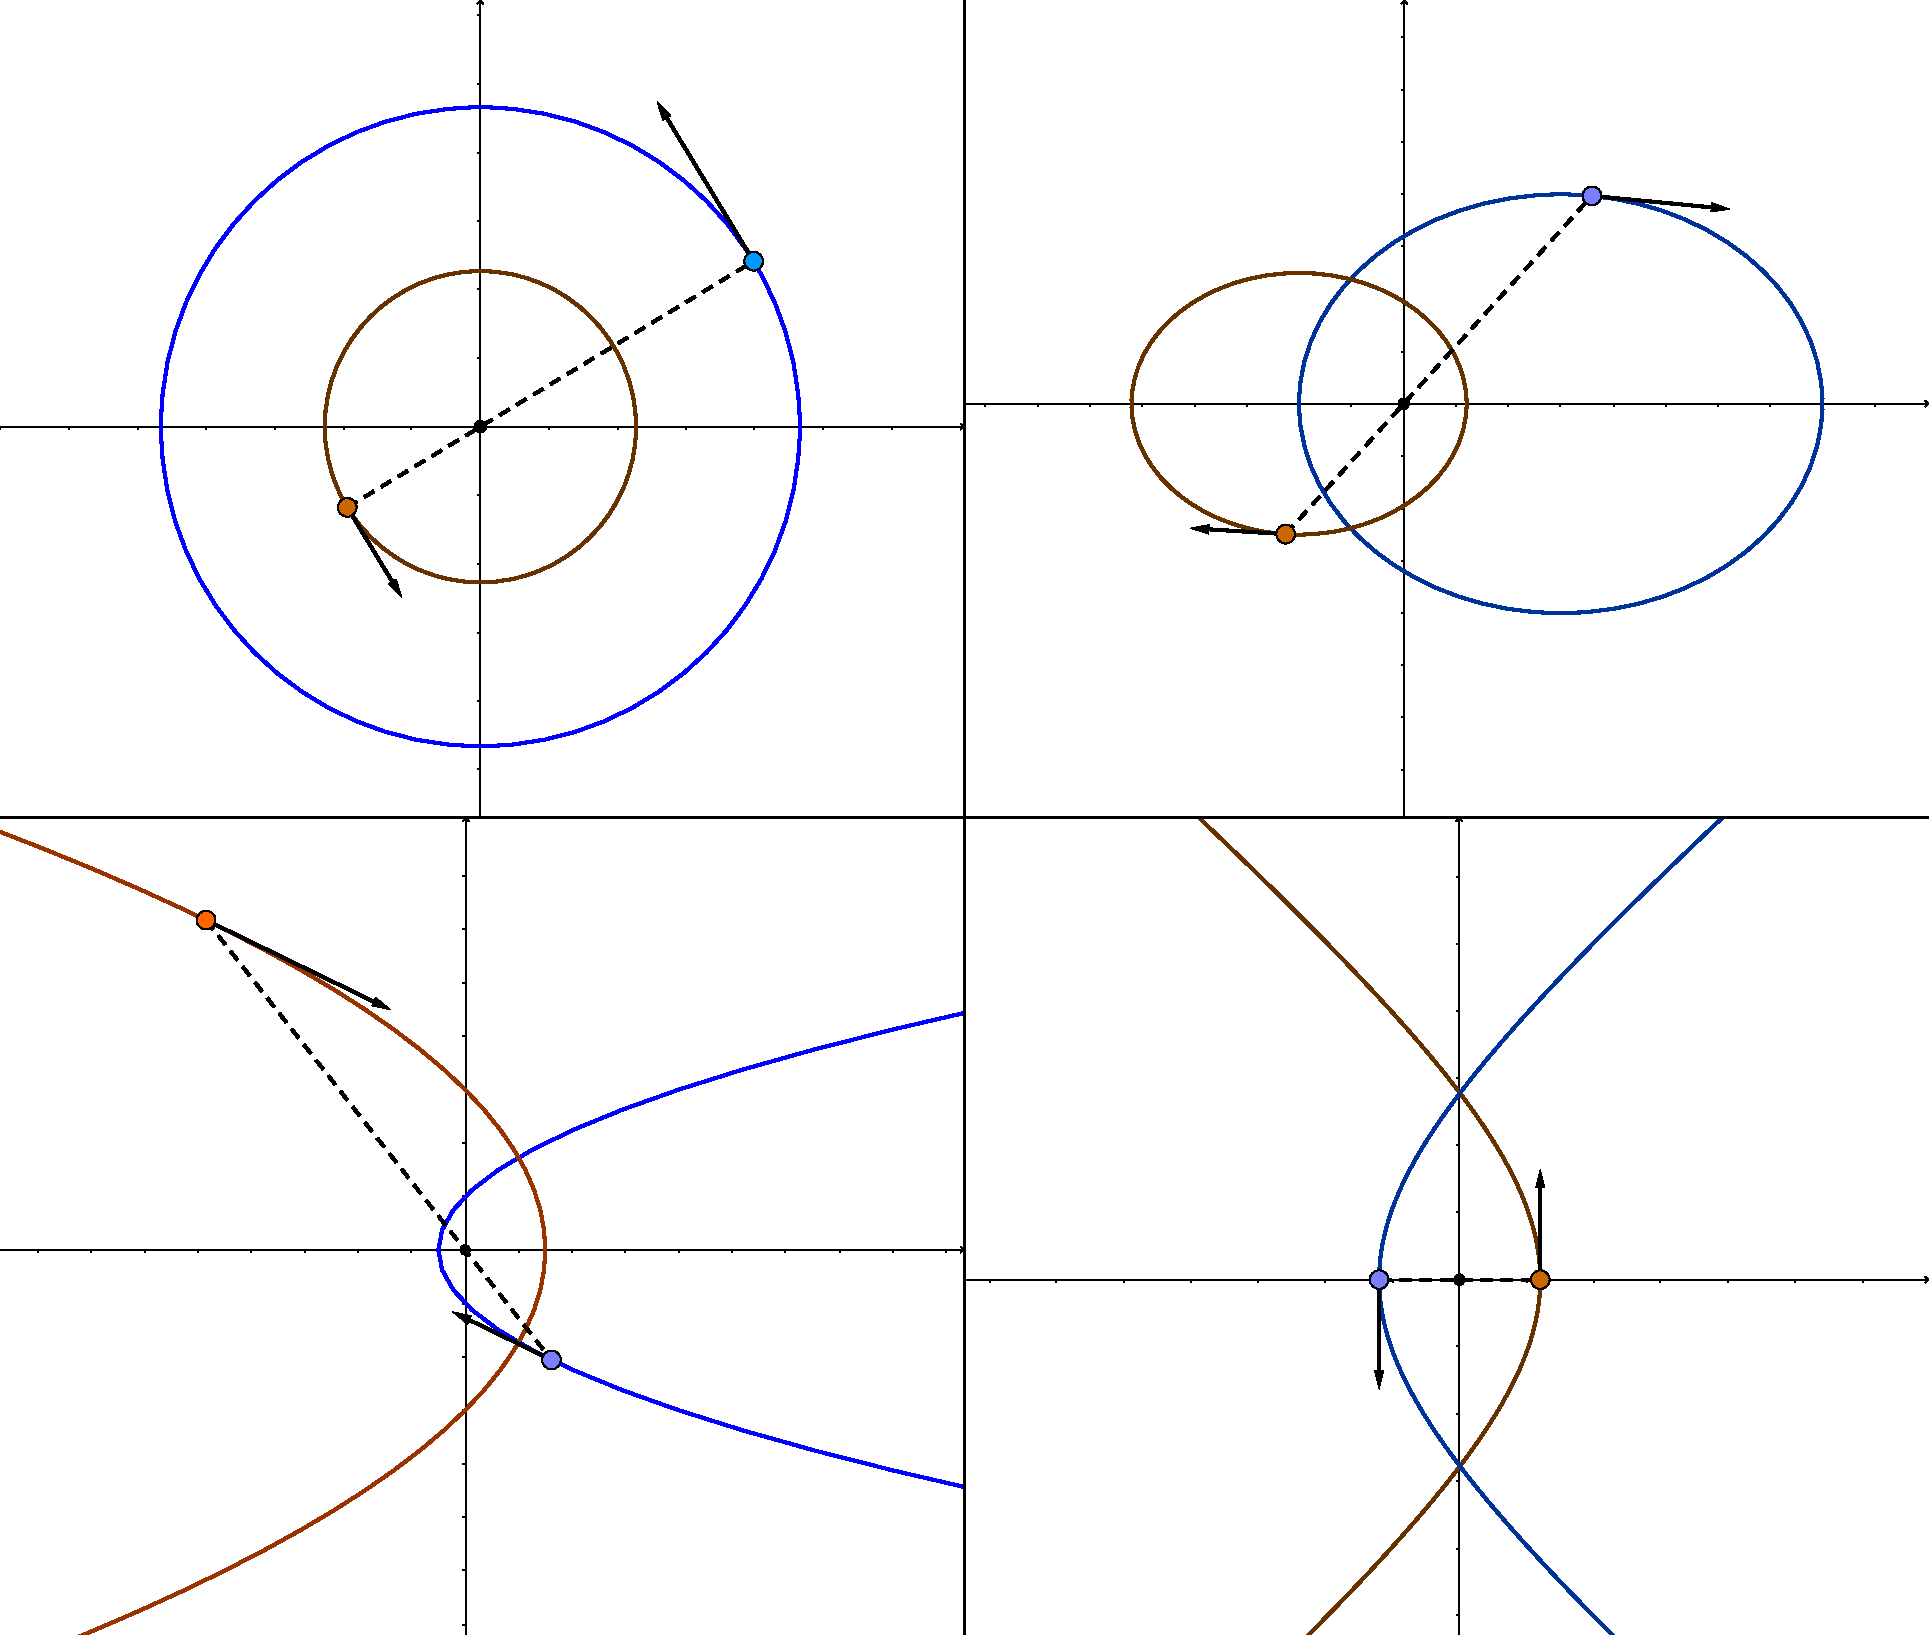
\includegraphics[width=14cm]{./figures/ConDB_2.pdf}
\caption{双体系统运动轨迹} \label{ConDB_fig2}
\end{figure}

若已知的轨迹上的一点,容易求出天体在该点处的速度矢量.对于天体M,可将速度矢量分解为切向速度 $v_\tau$ 与法向速度 $v_n$.在极坐标系中,切向速度可表示为 $v_\tau =r_1\vdot{\theta}$,而上文已证明守恒的系统角动量为
\begin{equation}\label{ConDB_eq10}
\bvec L  = m_1(1+\mu)\bvec r_1 \times \dot{\bvec r}_1= m_1(1+\mu)r_1^2\dot{\theta}\uvec z
\end{equation}
因此,切向速度为
\begin{equation}
v_\tau =\frac{L}{m_1(1+\mu)r_1}
\end{equation}

又因为法向速度 $v_n=\dot{\bvec r}_1$,对\autoref{ConDB_eq9} 求导可得
\begin{equation}
v_n =\dv{r_1}{t}=-\frac{ep\dot{\theta}\cos\theta}{(1+e\cos\theta)^2}=-\frac{epL\cos\theta}{m_1(1+\mu)r_1^2(1+e\cos\theta)^2}=-\frac{A_1\cos\theta}{m_1L}
\end{equation}

\subsection{时间参数}
通过对二体系统守恒量的分析,我们发现角动量和L-R-L矢量直接决定了轨道的形状和大小,再令极轴正方向与L-R-L矢量平行,则轨道方程在坐标系中就有唯一确定的表达式.以上的讨论中,我们避免了求解二阶运动微分方程的繁琐过程,然而美中不足的是,我们还没有建立天体运动的位置—时间关系式.下面就对时间参数展开讨论.

\autoref{ConDB_eq10} 通过角动量的定义式建立了轨道的角度参数和时间的关系,可以将该式改写为
\begin{equation}
\dv{\theta}{t}=\frac{L}{ m_1(1+\mu)r_1^2}
\end{equation}
将轨道方程\autoref{ConDB_eq9} 代入,并分离变量
\begin{equation}
\dd{t}=\frac{(1+\mu)L^3}{ m_1k^2}\frac{\dd{\theta}}{(1+e\cos\theta)}
\end{equation}
方程两边积分,可得
\begin{equation}\label{ConDB_eq15}
t-t_0 = \frac{(1+\mu)L^3}{ m_1k^2}\int_0^{\theta} \frac{\dd{\theta}}{(1+e\cos\theta)^2}
\end{equation}
其中 $t_0$ 为初始时间,习惯上取 $\theta=0$ 的时刻为时间的零点,即 $t_0=0$ .等号右边的积分根据轨道形状有不同的表达式,以圆形和抛物线为例
\begin{equation}
\int_0^{\theta} \frac{\dd{\theta}}{(1+e\cos\theta)^2} =
\leftgroup{
&\theta &(e=0)\\
&\frac{1}{2}\tan(\frac{\theta}{2})+\frac{1}{6}\tan[3](\frac{\theta}{2}) &(e=1)
} 
\end{equation}
对应椭圆和双曲线的积分表达式非常复杂,有需要的读者可查阅标准数学手册积分表.

由于\autoref{ConDB_eq15} 中的被积函数在其有效定义域上为正值,因此所得的时间 $t$ 单调递增,即 $\theta$ 与 $t$ 存在一一对应的关系.

综上所述,可以得出结论:\textbf{二体系统的运动问题在给定的初始条件下具有确定解}.

\begin{exercise}{关于系统机械能}\label{ConDB_exe1}
试证明二体系统机械能守恒.

提示:可以选用以下两种方法
\begin{itemize}
\item 写出天体M和N的二阶运动微分方程,分别与其速度矢量内积;
\item 系统机械能等于动能与引力势能的和,写出机械能表达式并适当代换,最终可用角动量和L-R-L矢量表达系统机械能.
\end{itemize}
\end{exercise}
